\vspace{-3em}

\begin{IEEEbiography}[{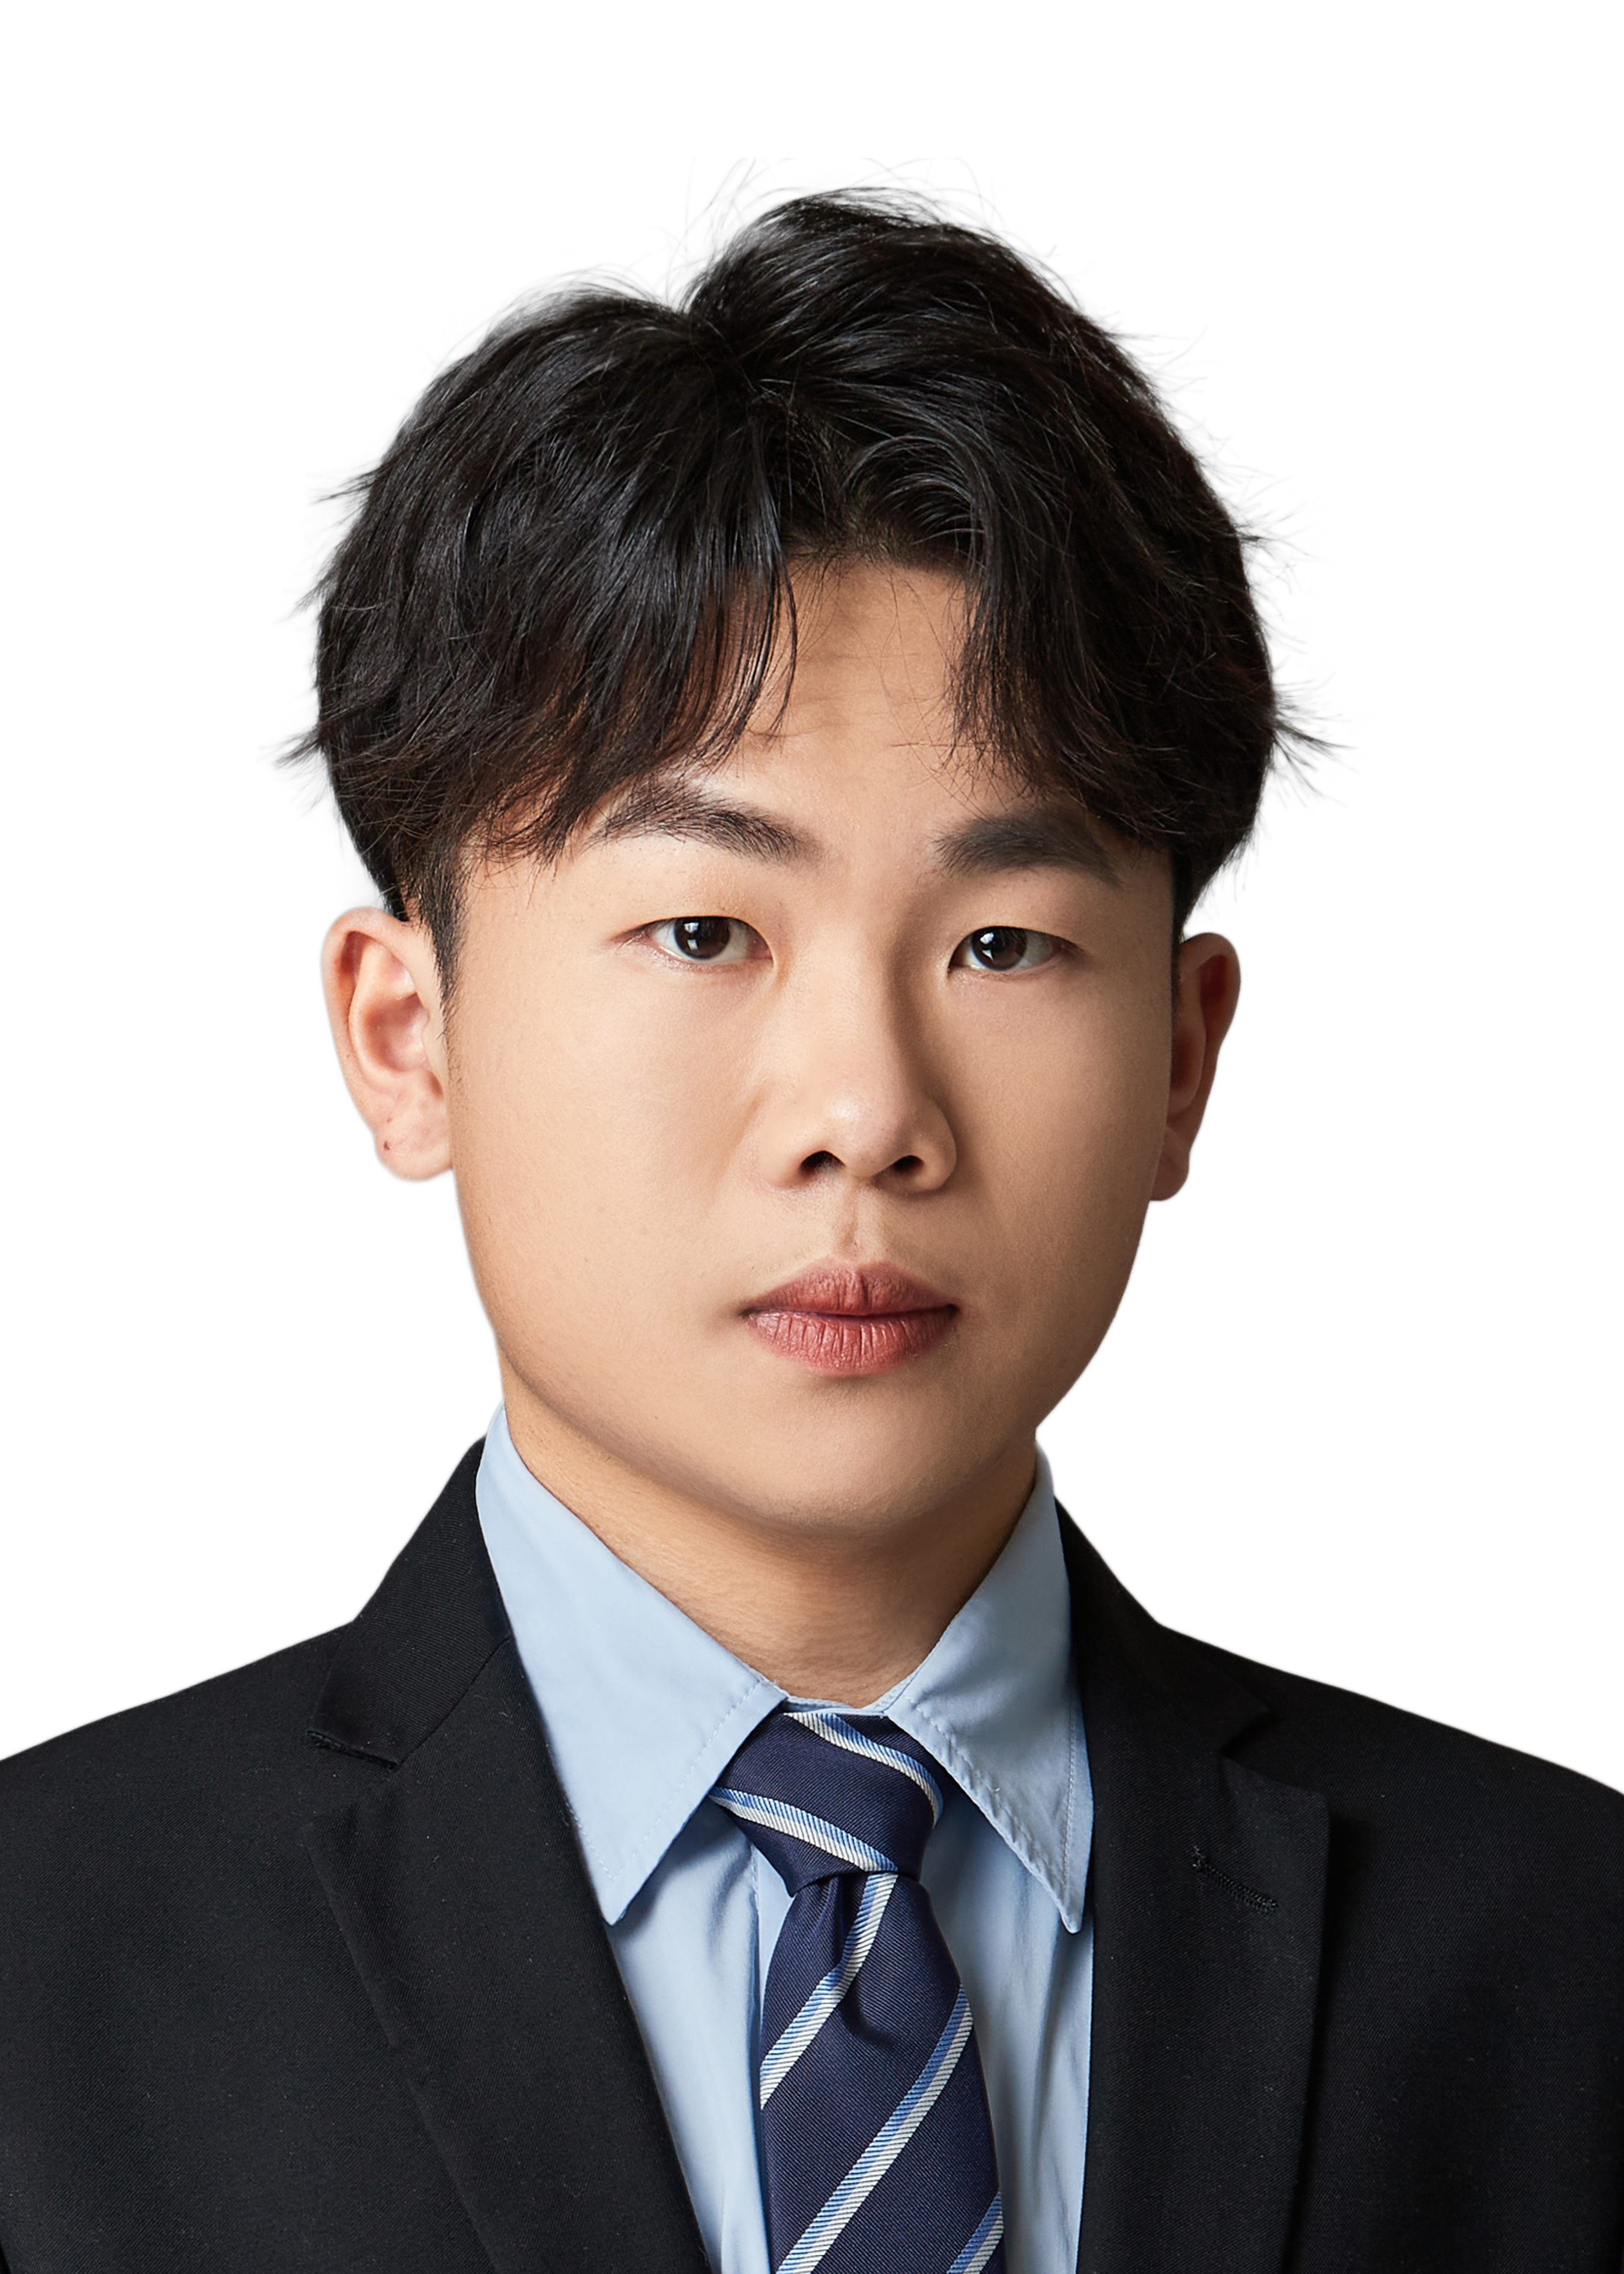
\includegraphics[width=1in,height=1.25in,clip,keepaspectratio]{id_photos/Guangyi_Liu.jpg}}]{Guangyi Liu}
received the B.Eng. degree from China University of Mining and Technology, Xuzhou, China, in 2023. He is currently pursuing the M.S. degree in the College of Information Science and Electronic Engineering at Zhejiang University, Hangzhou, China. His research interests include large language model.
\end{IEEEbiography}

\vspace{-3em}

\begin{IEEEbiography}[{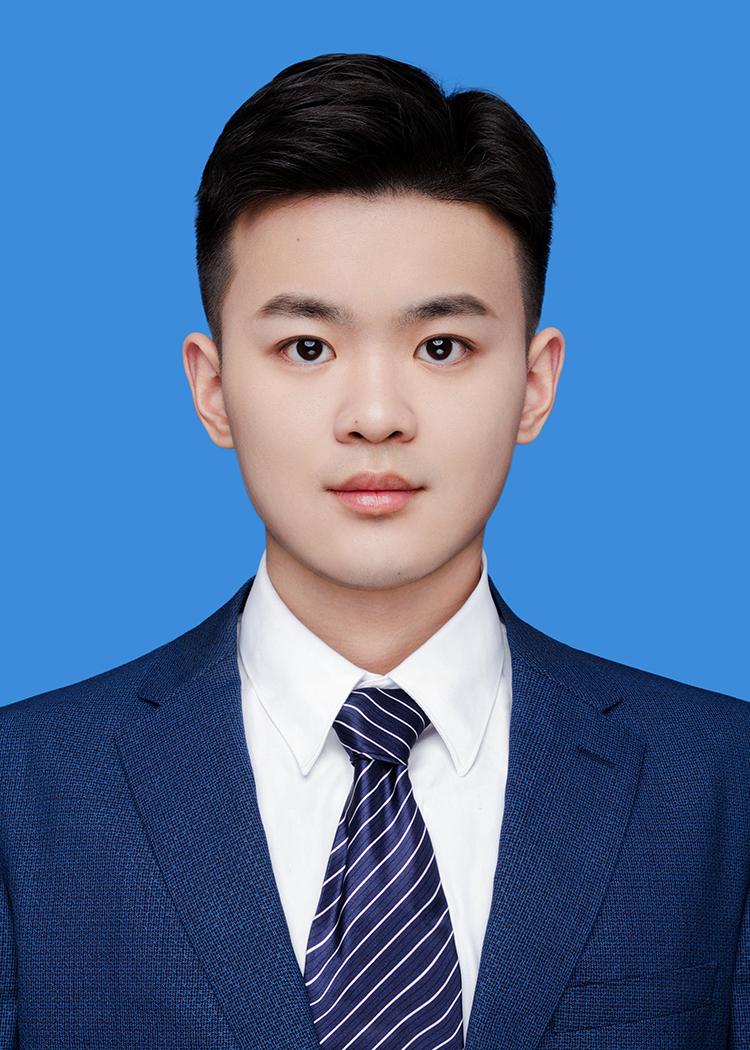
\includegraphics[width=1in,height=1.25in,clip,keepaspectratio]{id_photos/Pengxiang_Zhao.jpg}}]{Pengxiang Zhao}
received the BS degree in automation from the Huazhong Agricultural University, Wuhan, China, in 2024. He is currently working toward the MS degree with the Institute of Cyber-Systems and Control, Advanced Perception on Robotics and Intelligent Learning Lab (APRIL), Zhejiang University, China, under the supervision of Dr. Yong Liu. His primary research interests include LLM and AI agent.
\end{IEEEbiography}

\vspace{-3em}

\begin{IEEEbiography}[{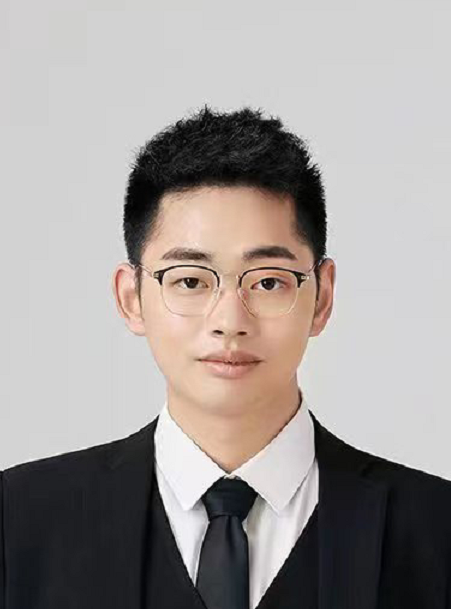
\includegraphics[width=1in,height=1.25in,clip,keepaspectratio]{id_photos/Liang_Liu.png}}]{Liang Liu}
received a Ph.D. degree in control science and engineering from Zhejiang University in 2021. He is currently a researcher at the vivo AI Lab. His current research interests include AI Agents, Multimodal LLMs, and Computer Vision. He has authored and co-authored approximately 50 papers published in top-tier academic journals and conferences, including T-PAMI, T-NNLS, T-IP, T-MM, CVPR, ICCV, AAAI, IJCAI, ACM MM, etc. He has also served as a reviewer for numerous academic journals and conferences.
\end{IEEEbiography}

\vspace{-3em}

\begin{IEEEbiography}[{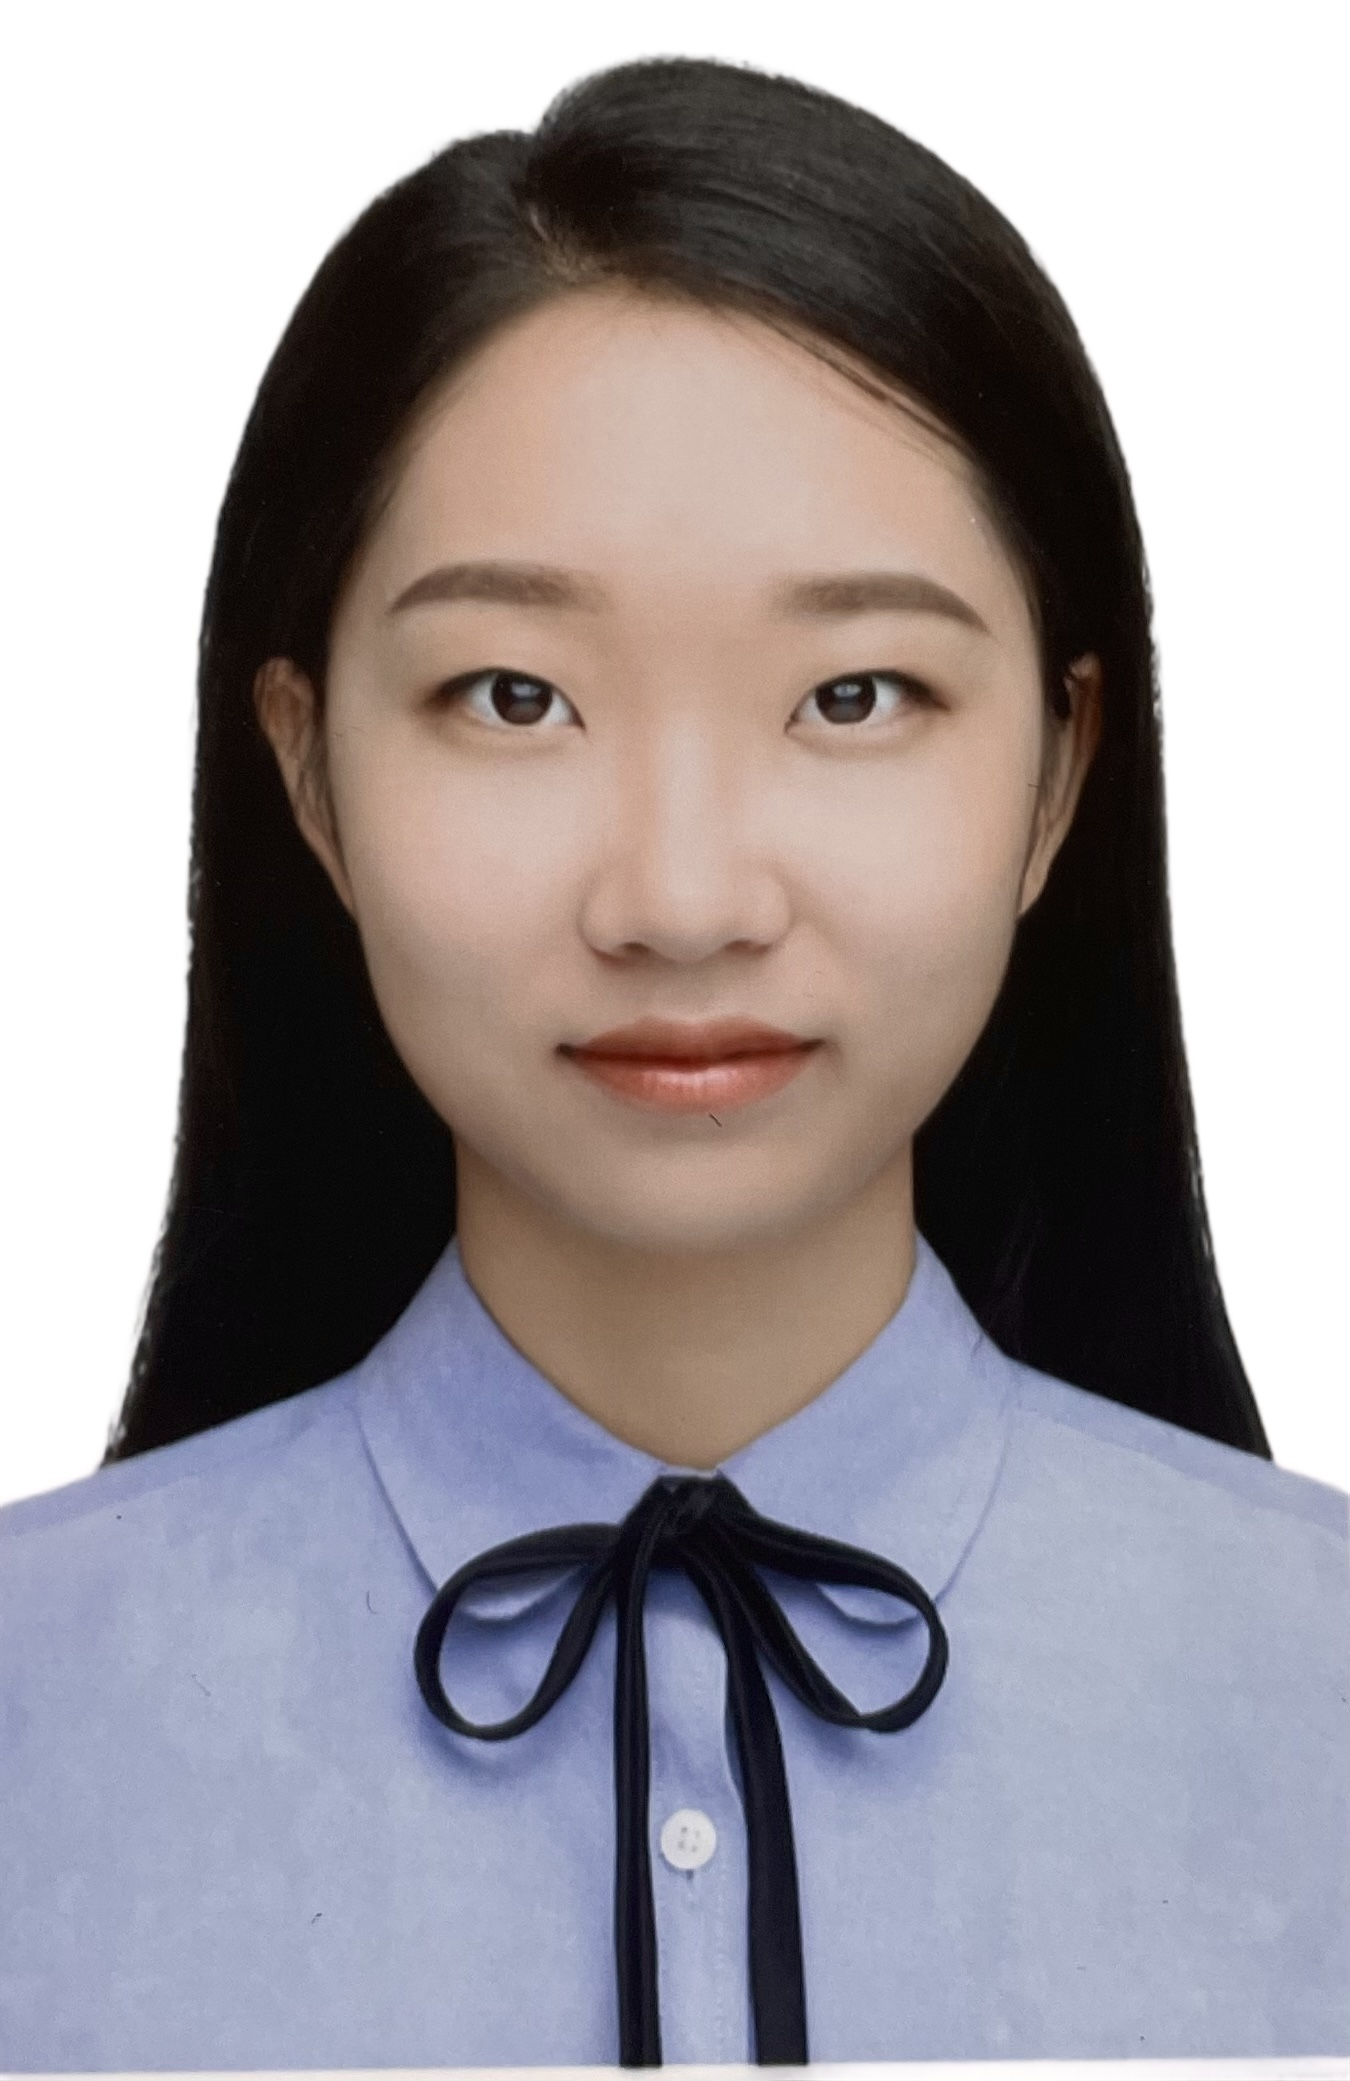
\includegraphics[width=1in,height=1.25in,clip,keepaspectratio]{id_photos/Yaxuan_Guo.jpg}}]{Yaxuan Guo}
received the Master Degree from University of Waterloo, Canada, in 2020 and the Bachelor Degree from Hong Kong Baptist University, Hong Kong, in 2018. She is currently a Machine Learning Engineer in vivo AI Lab. Her research interests include GUI Agent, machine learning and reinforcement learning.
\end{IEEEbiography}

\vspace{-3em}

\begin{IEEEbiography}[{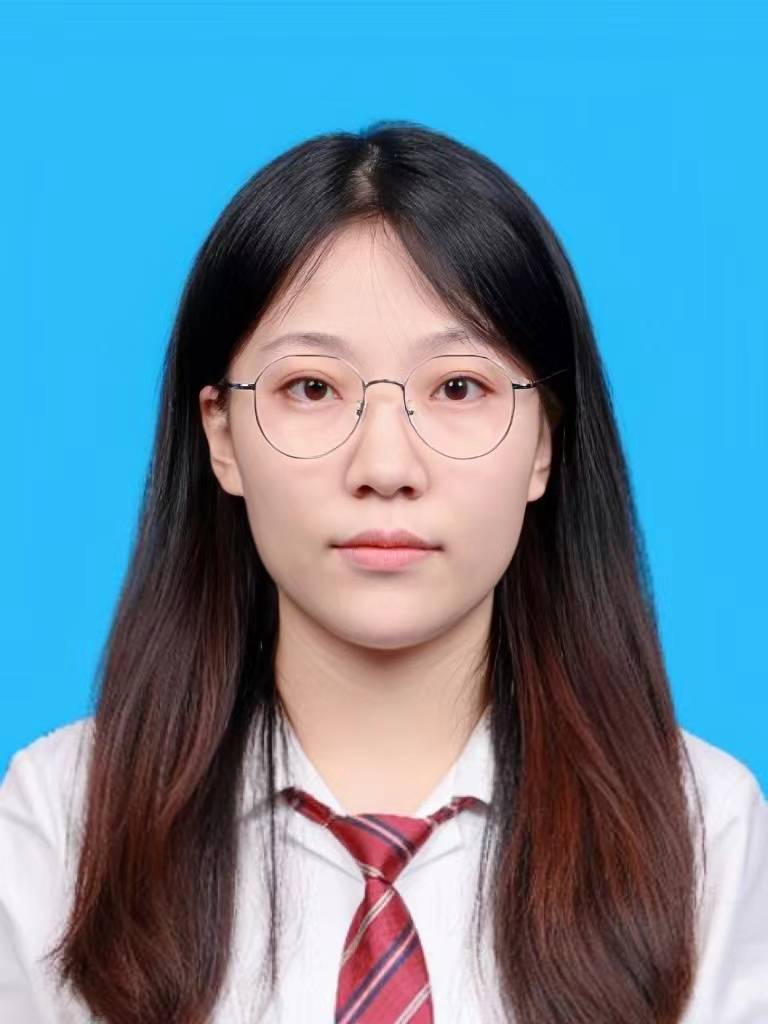
\includegraphics[width=1in,height=1.25in,clip,keepaspectratio]{id_photos/Han_Xiao.jpeg}}]{Han Xiao}
is currently pursuing the Ph.D. degree with The Chinese University of Hong Kong, Hong Kong, since 2023. She received her M.S. degree from Tsinghua University, Beijing, China, in 2023, and her B.S. degree from Tsinghua University in 2020. Her research interests include computer vision and multimodal large language models. She has published several papers in top-tier conferences and journals, including TPAMI/CVPR/ICCV/NeurIPS. She serves as a reviewer for several international conferences and journals.
\end{IEEEbiography}

\vspace{-3em}

\begin{IEEEbiography}[{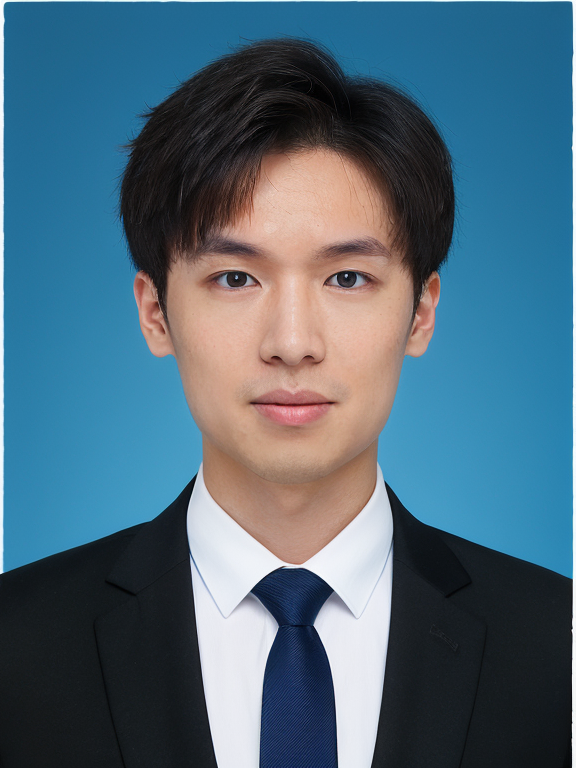
\includegraphics[width=1in,height=1.25in,clip,keepaspectratio]{id_photos/Weifeng_Lin.png}}]{Weifeng Lin}
earned his Bachelor's and Master's degrees at South China University of Technology, majoring in Electronic Information and Technology. He will commence his Ph.D. studies at The Chinese University of Hong Kong in 2025. His research primarily focuses on deep learning and computer vision, including multimodal generation and understanding. He has published first-author papers at several top-tier international conferences.
\end{IEEEbiography}

\vspace{-3em}

\begin{IEEEbiography}[{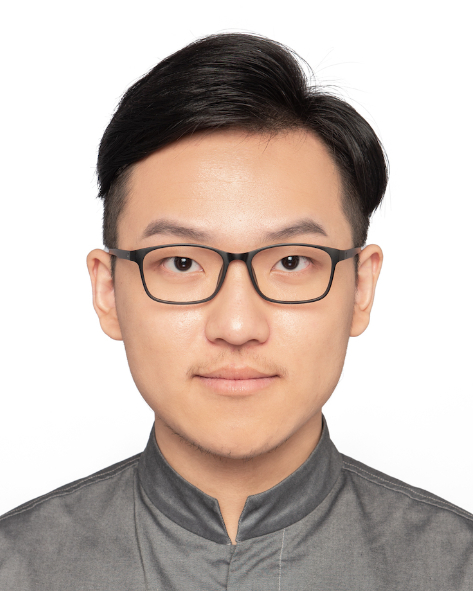
\includegraphics[width=1in,height=1.25in,clip,keepaspectratio]{id_photos/Yuxiang_Chai.jpg}}]{Yuxiang Chai}
received the BS and MS degrees in computer science from New York University, New York City, USA, in 2021 and 2023 respectively. He is currently a PhD candidate student at the Chinese University of Hong Kong. His research interests include large language model, machine learning, deep learning.
\end{IEEEbiography}

\vspace{-3em}

\begin{IEEEbiography}[{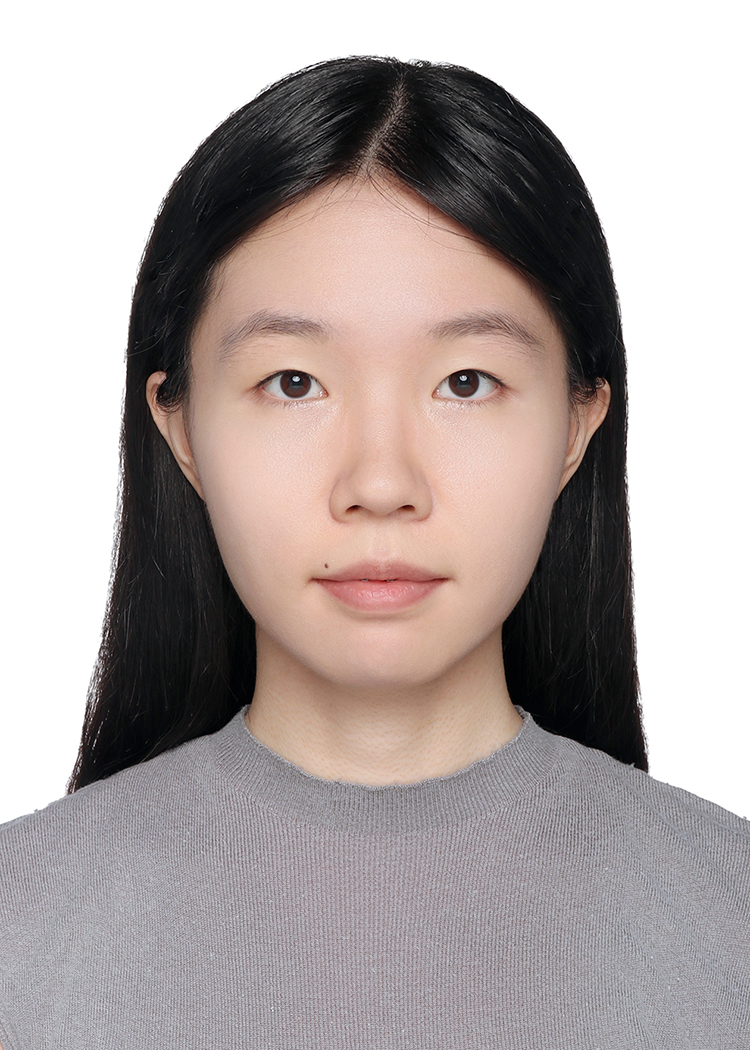
\includegraphics[width=1in,height=1.25in,clip,keepaspectratio]{id_photos/Yue_Han.jpg}}]{Yue Han}
is currently pursuing a Ph.D. degree at the Institute of Cyber-Systems and Control, Advanced Perception on Robotics and Intelligent Learning Lab (APRIL), Zhejiang University, China, under the supervision of Dr. Yong Liu. She earned her B.Eng. degree in Automation from the School of Southeast University, Nanjing, China, in 2021. Her primary research interests include computer vision, few-shot instance segmentation, and talking face generation.
\end{IEEEbiography}

\vspace{-3em}

\begin{IEEEbiography}[{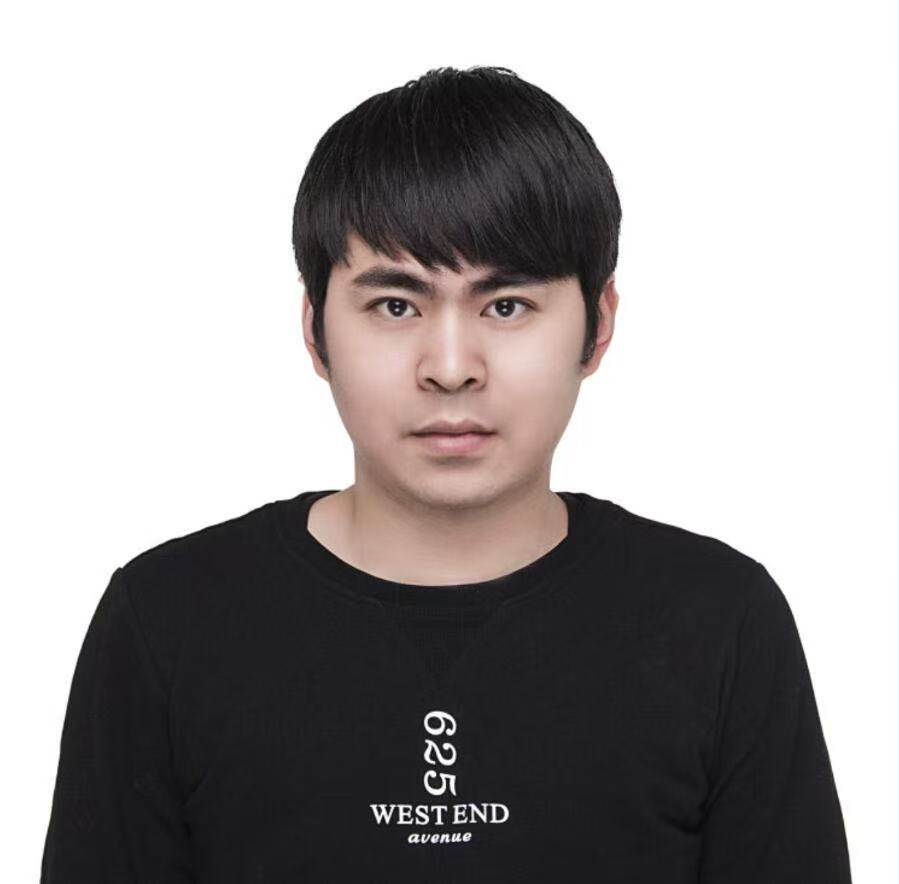
\includegraphics[width=1in,height=1.25in,clip,keepaspectratio]{id_photos/Shuai_Ren.jpg}}]{Shuai Ren}
received his bachelor's degree in electronic information science and technology from Lanzhou University in 2012 and his master's degree in signal and information processing from Lanzhou University in 2015. He is currently a vivo algorithm expert. His research interests include computer vision, multimodal large models, and machine learning.
\end{IEEEbiography}

\vspace{-3em}

\begin{IEEEbiography}[{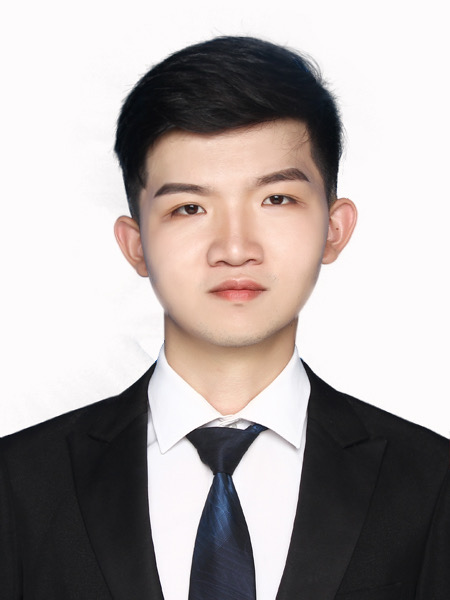
\includegraphics[width=1in,height=1.25in,clip,keepaspectratio]{id_photos/Hao_Wang_ZJU.jpeg}}]{Hao Wang}
is a Ph.D. candidate in the State Key Laboratory of Industrial Control Technology, Zhejiang University, Hangzhou, China. 
His research interests span from time-series analysis, causal machine learning and recommendation systems.
He has published more than 20 papers in top-tier AI conferences and journals such as ICML, NeurIPS, ICLR, AAAI, SIGKDD, WWW, SIGIR, TKDE, etc.
Moreover, he has been served as the reviewer for several top conferences including ICML, NeurIPS, ICLR, SIGKDD, WWW.
\end{IEEEbiography}

\vspace{-3em}

\begin{IEEEbiography}[{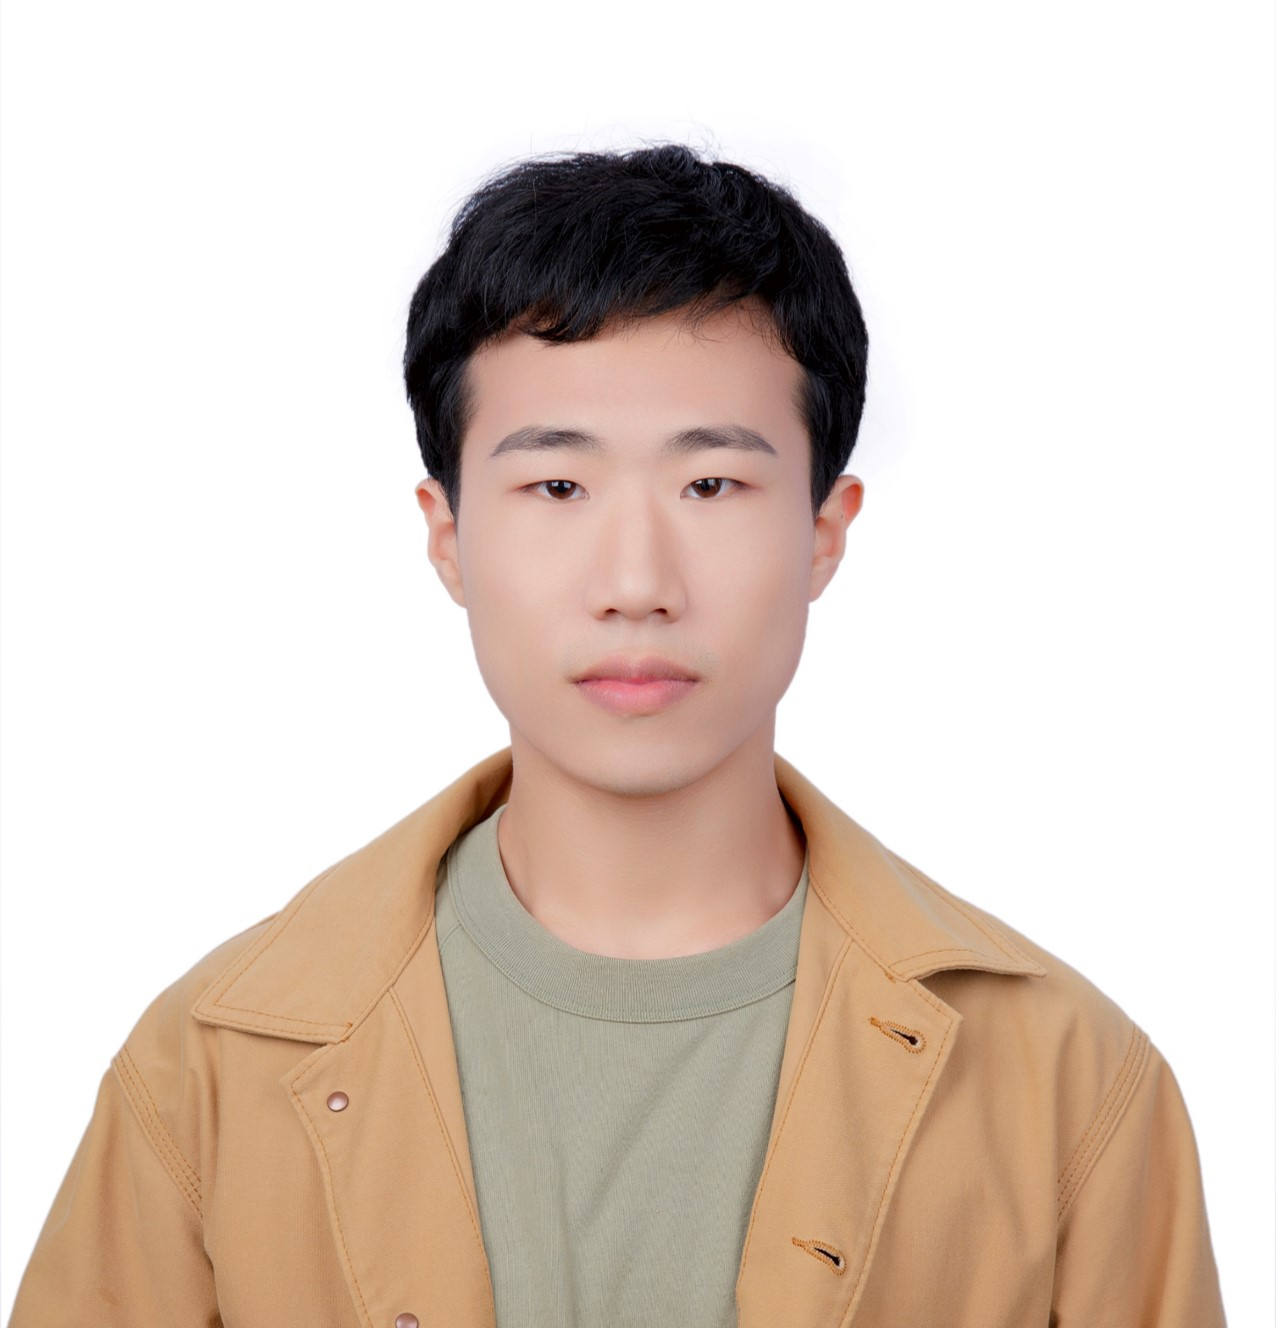
\includegraphics[width=1in,height=1.25in,clip,keepaspectratio]{id_photos/Xiaoyu_Liang.jpg}}]{Xiaoyu Liang}
received the B.S. degree from Zhejiang University, Hangzhou, Zhejiang, China, in 2022, and received the M.S. degree from the same institution in 2025. His current research interests include Multimodal Large Language Models, Agents, and Model Compression.
\end{IEEEbiography}

\vspace{-3em}

\begin{IEEEbiography}[{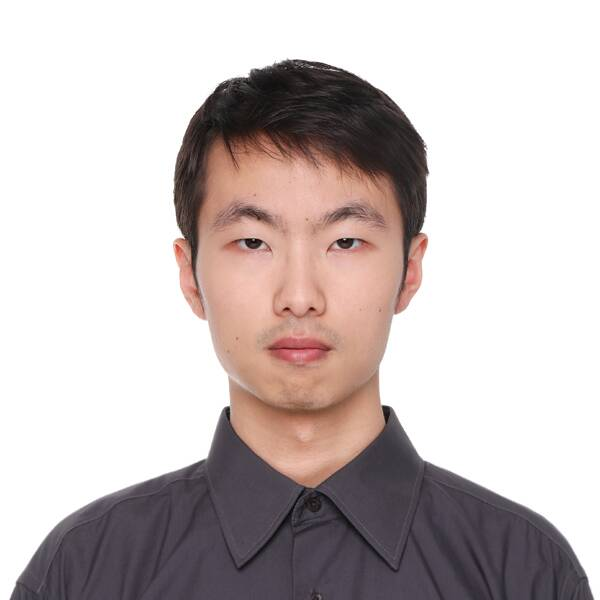
\includegraphics[width=1in,height=1.25in,clip,keepaspectratio]{id_photos/Wenhao_Wang.jpg}}]{Wenhao Wang}
received the B.S. degree in Cyberspace Security from WHU University, City, China, in 2023. He is currently working toward the Ph.D. degree in Computer Science with Zhejiang University, City, China. His research interests include GUI Agents, Federated Learning, Large language models.
\end{IEEEbiography}

\vspace{-3em}

\begin{IEEEbiography}[{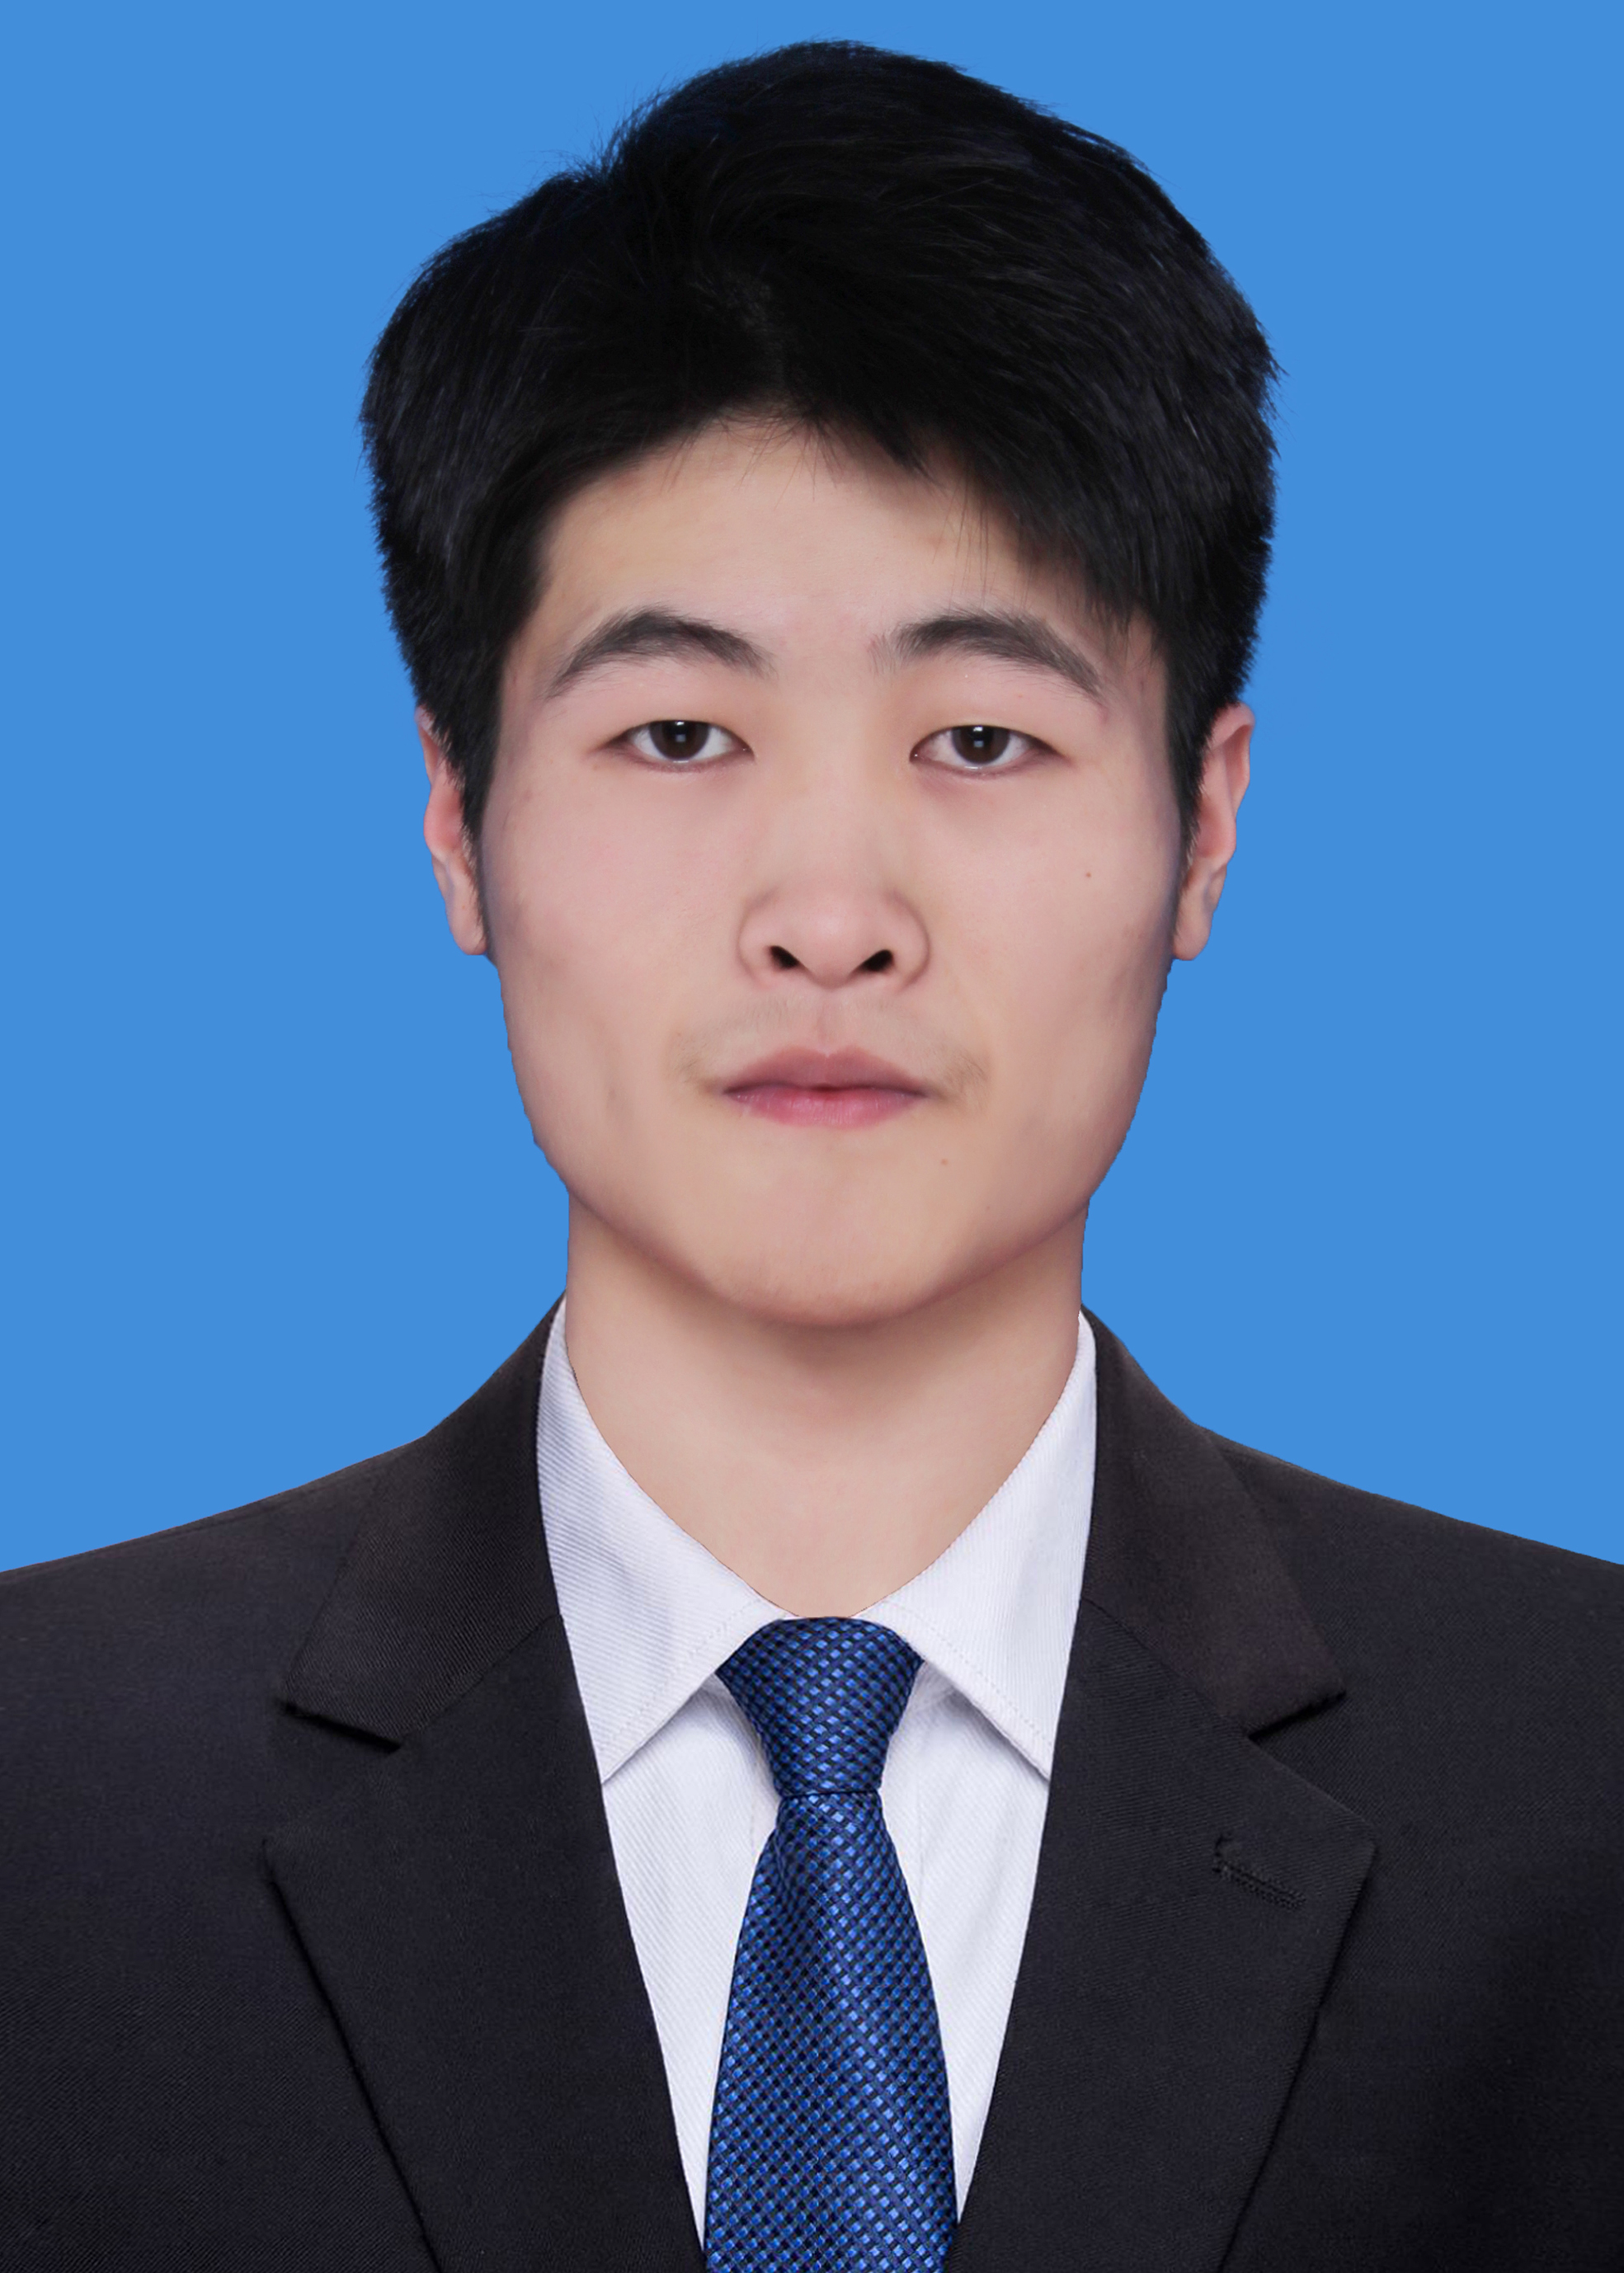
\includegraphics[width=1in,height=1.25in,clip,keepaspectratio]{id_photos/Tianze_Wu.jpg}}]{Tianze Wu}
received the B.Eng. degree from China University of Mining and Technology, Xuzhou, China, in 2023. He is currently pursuing the M.S. degree in the College of Information Science and Electronic Engineering at Zhejiang University, Hangzhou, China. His research interests include large language model.
\end{IEEEbiography}

\vspace{-3em}

\begin{IEEEbiography}[{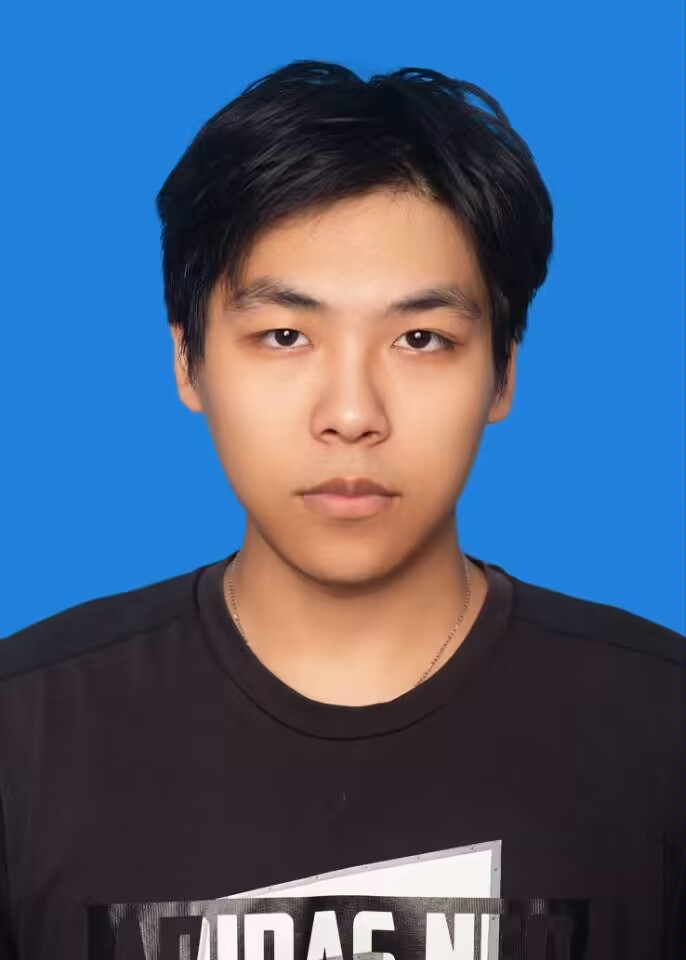
\includegraphics[width=1in,height=1.25in,clip,keepaspectratio]{id_photos/Linghao_Li.jpg}}]{Linghao Li}
studied in the School of Software Technology, Zhejiang University, where he researched the direction of Retrieval Augmented Generation.
\end{IEEEbiography}

\vspace{-3em}

\begin{IEEEbiography}[{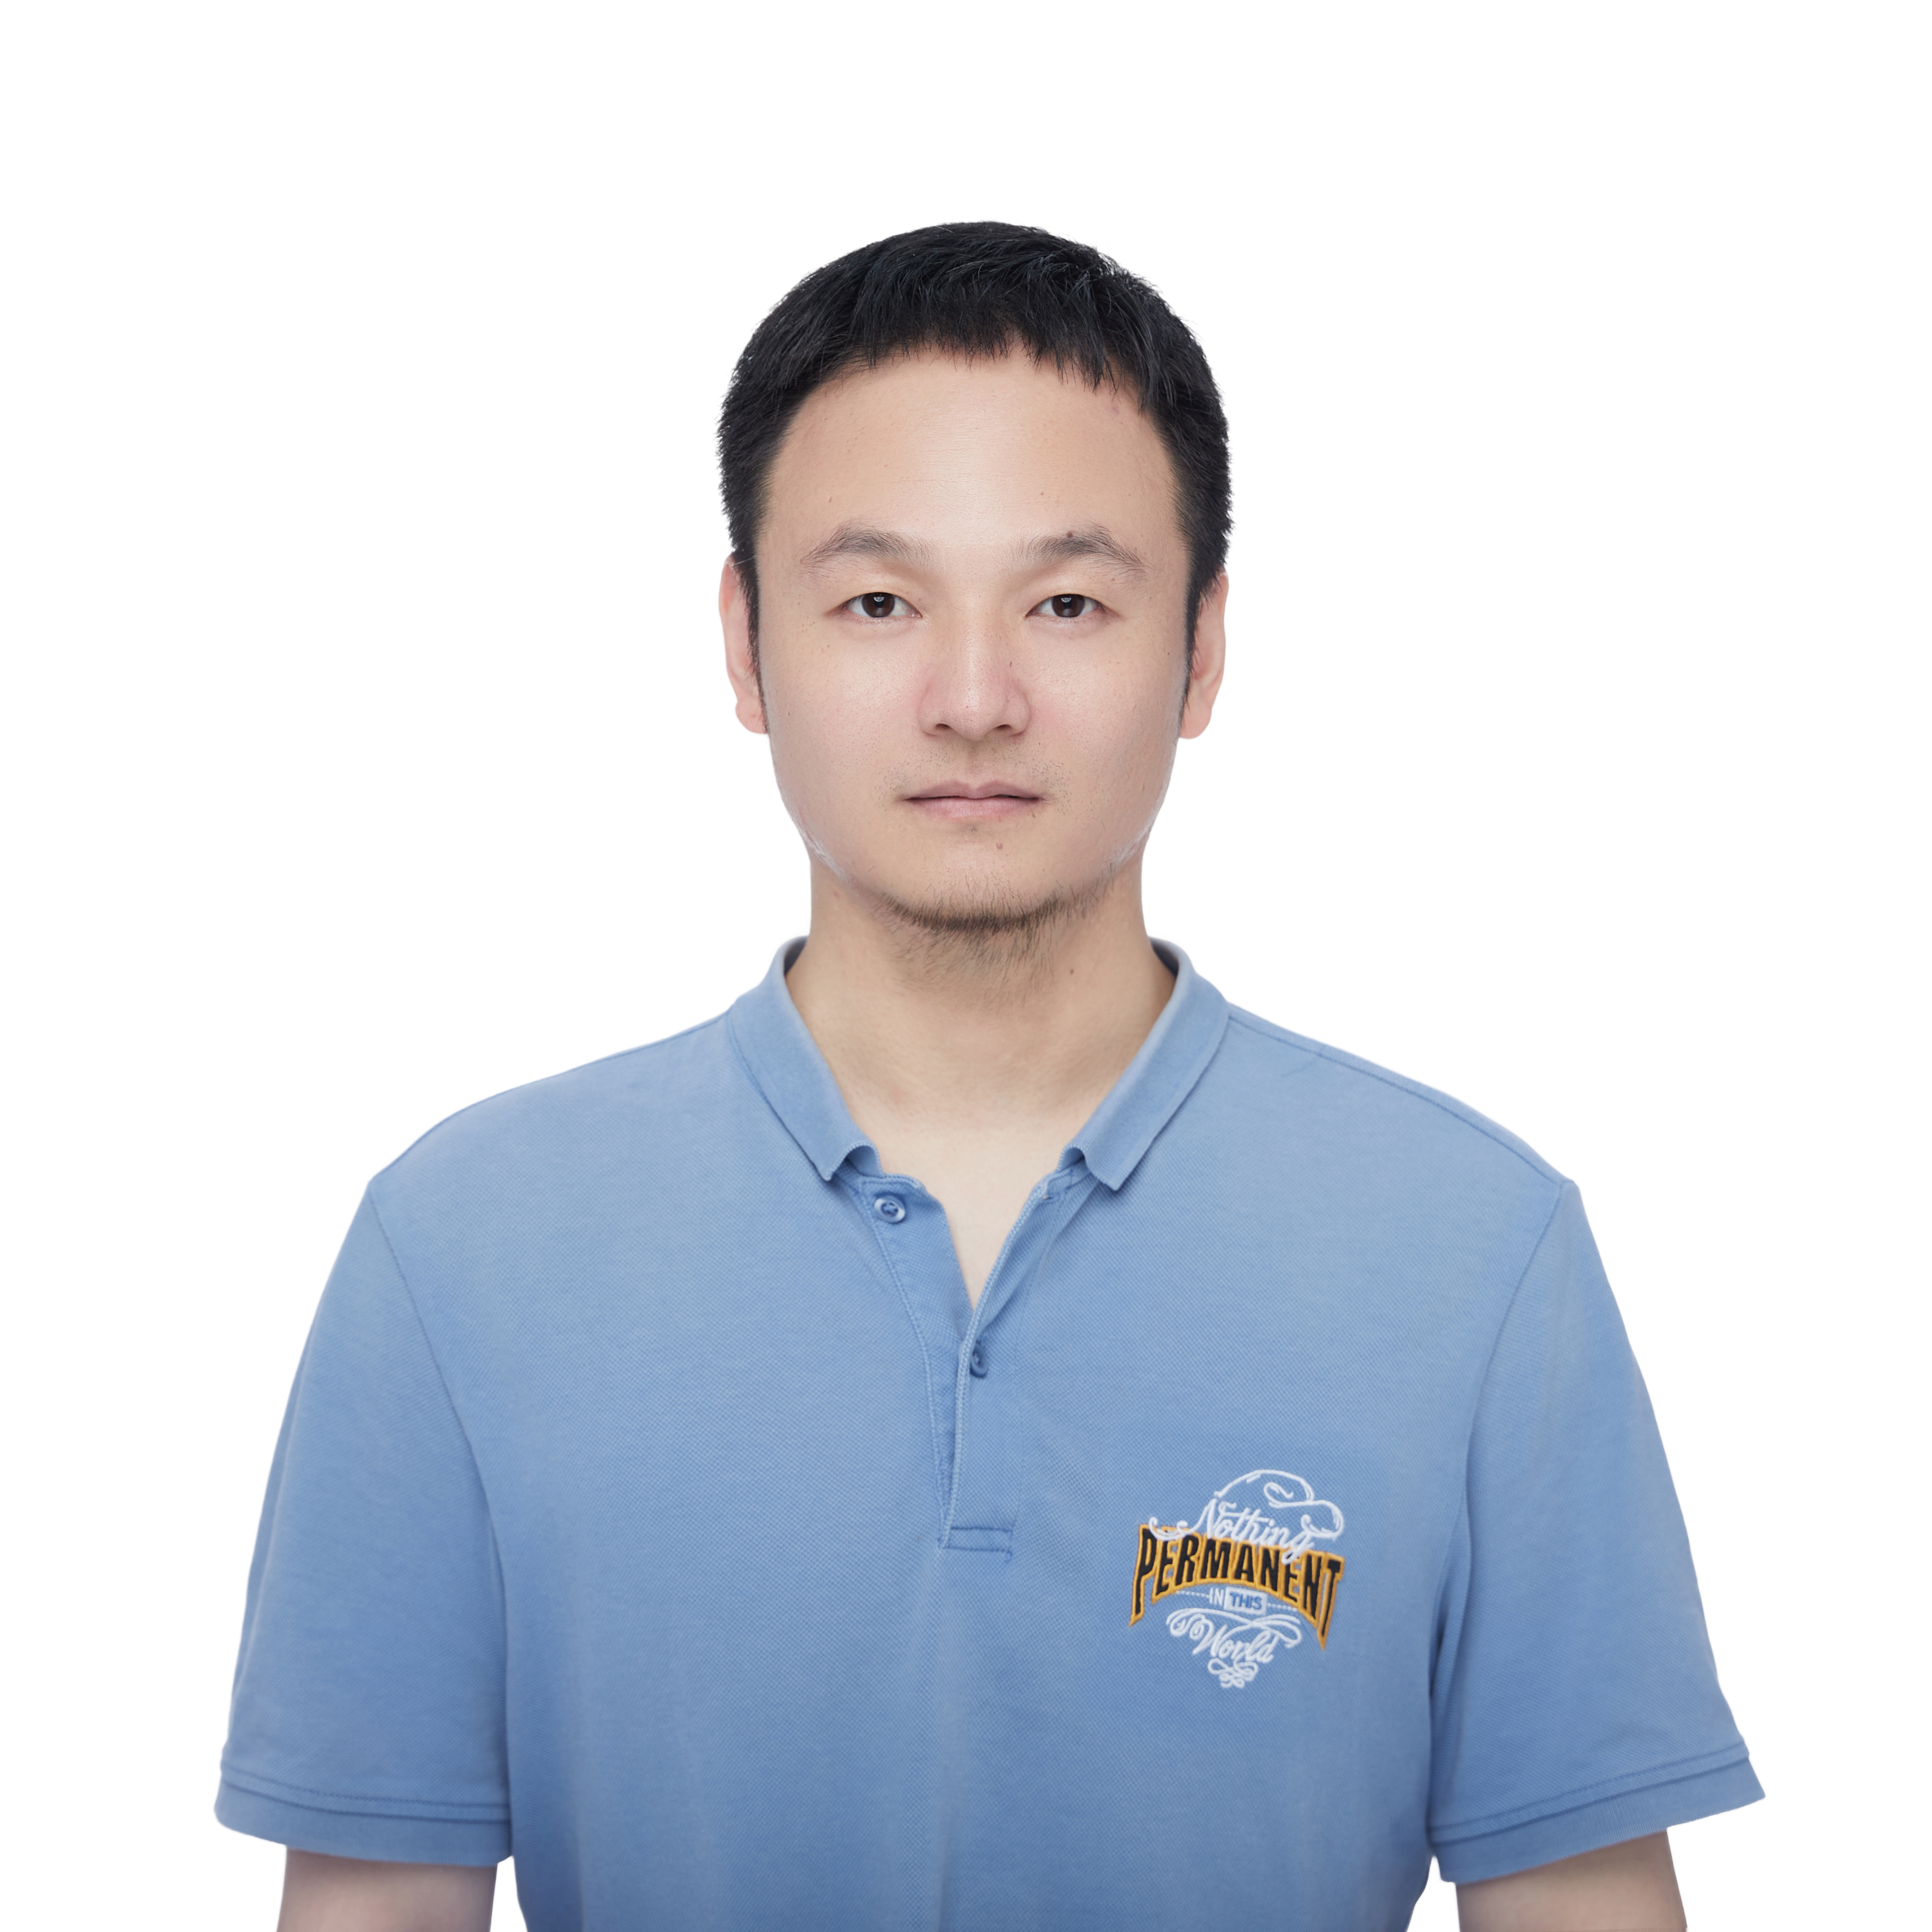
\includegraphics[width=1in,height=1.25in,clip,keepaspectratio]{id_photos/Hao_Wang_vivo.jpg}}]{Hao Wang}
received his PHD in Mechanical Engineering at Arizona State University. He now works at Vivo on AI agents.
\end{IEEEbiography}

\vspace{-3em}

\begin{IEEEbiography}[{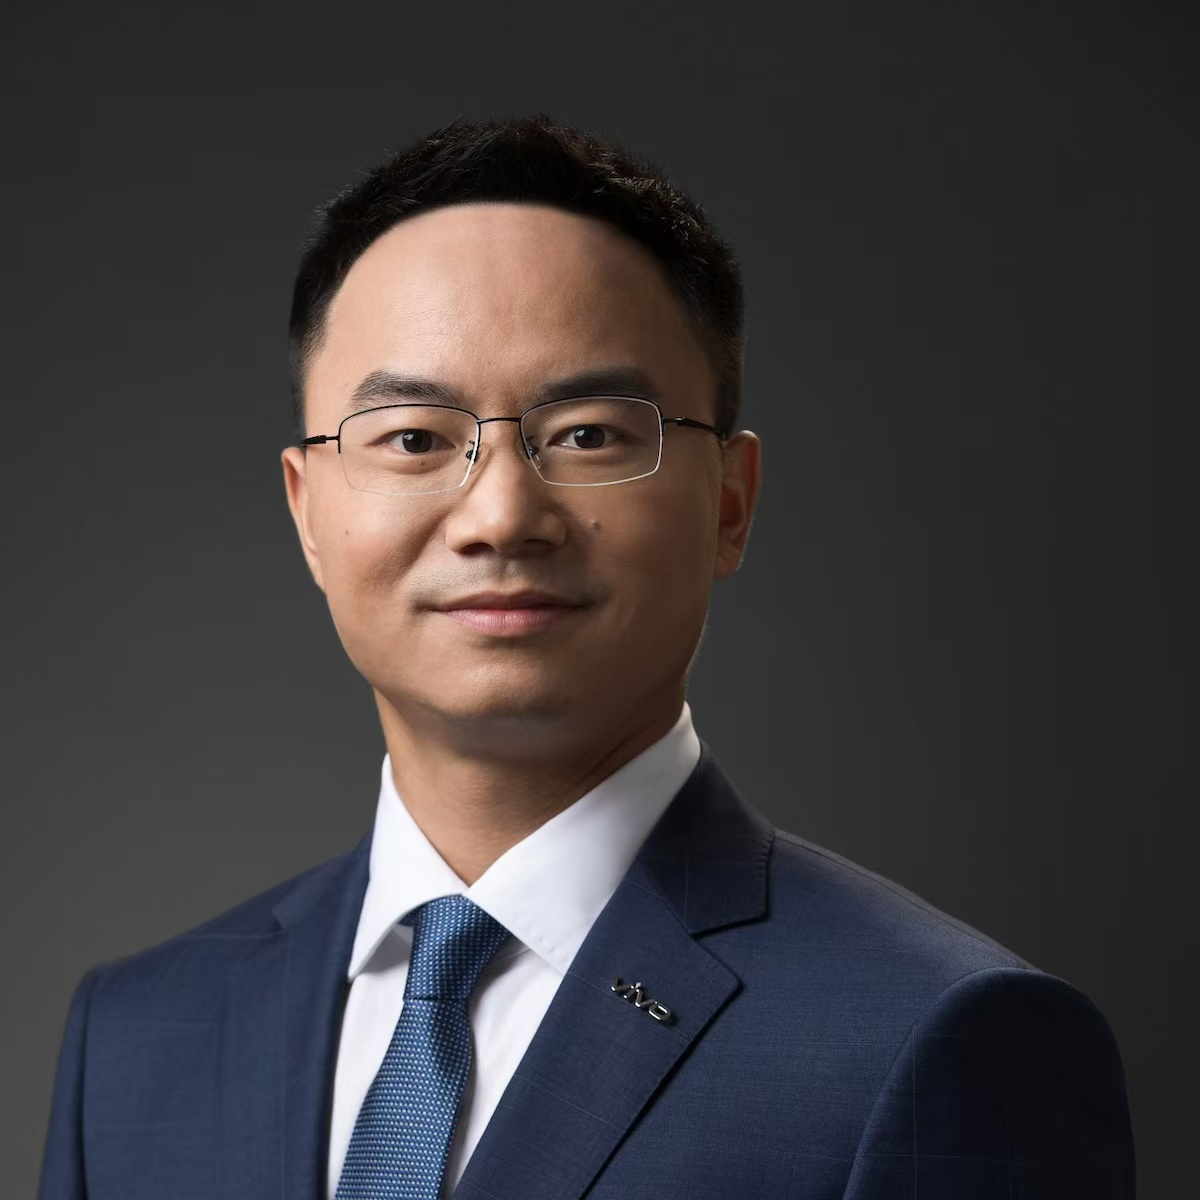
\includegraphics[width=1in,height=1.25in,clip,keepaspectratio]{id_photos/Guanjing_Xiong.jpg}}]{Guanjing Xiong}
received an M.S. degree from Wuhan University, China, in 2016. Currently at vivo AI Lab, his research focuses on on-device AI, proactive intelligence, and AI Agents. With his academic and practical experience, he drives the application of cutting-edge AI in mobile devices, aiming to deliver intelligent and convenient user experiences.
\end{IEEEbiography}

\vspace{-3em}

\begin{IEEEbiography}[{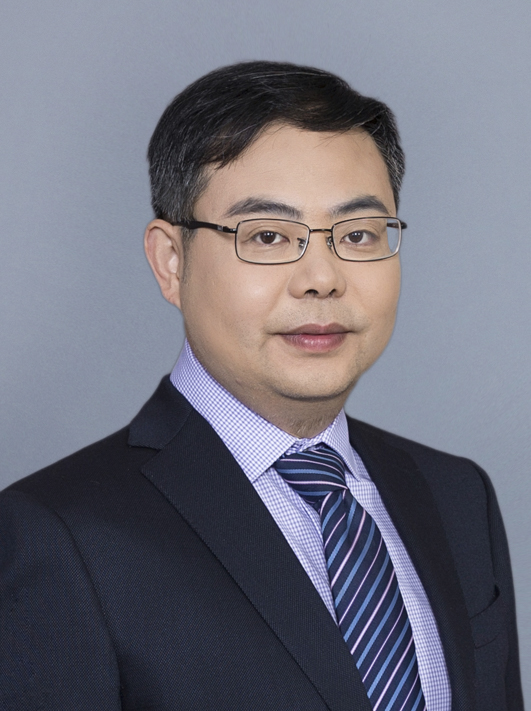
\includegraphics[width=1in,height=1.25in,clip,keepaspectratio]{id_photos/Yong_Liu.jpg}}]{Yong Liu}
received the BS degree in computer science and engineering and the PhD degree in computer science from Zhejiang University, Zhejiang, China, in 2001 and 2007, respectively. He is currently a professor with the Institute of Cyber-Systems and Control, Zhejiang University. His main research interests include: robot perception and vision, deep learning, Big Data analysis, and multi-sensor fusion. His research interests on machine learning, computer vision, information fusion, and robotics.
\end{IEEEbiography} 

\vspace{-3em}

\begin{IEEEbiography}[{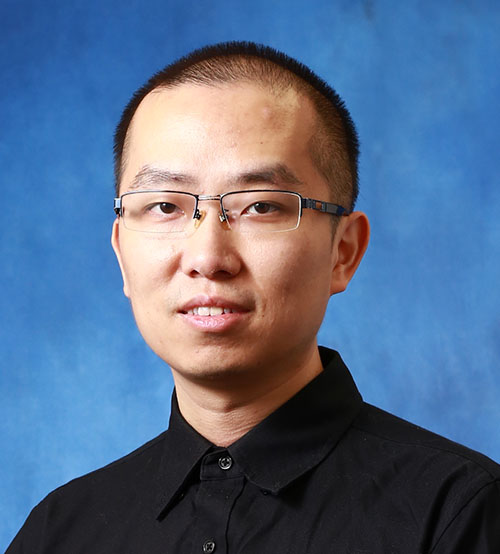
\includegraphics[width=1in,height=1.25in,clip,keepaspectratio]{id_photos/Hongsheng_Li.jpg}}]{Hongsheng Li}
received the BS degree in automation from the East China University of Science and Technology, Shanghai, China, in 2006, and the MS and PhD degrees in computer science from Lehigh University, Bethlehem, Pennsylvania, in 2010 and 2012, respectively. He is currently an associate professor with the Department of Electronic Engineering, Chinese University of Hong Kong. His research interests include computer vision, medical image analysis, and machine learning.
\end{IEEEbiography}

